\documentclass[10pt, oneside]{article}

\usepackage{amsmath}
\usepackage{amsthm}
\usepackage{amssymb}
\usepackage{calrsfs}
\usepackage{wasysym}
\usepackage{verbatim}
\usepackage{bbm}
\usepackage{color}
\usepackage{graphics}
\usepackage{geometry}
\usepackage{graphicx}

% for tables
\usepackage{booktabs}
\usepackage{siunitx}

% \usepackage{natbib} % For bibliography management
\usepackage[numbers]{natbib}
\usepackage{hyperref} % For clickable references


\geometry{tmargin=.75in, bmargin=.75in, lmargin=.75in, rmargin = .75in}  

\newcommand{\R}{\mathbb{R}}
\newcommand{\C}{\mathbb{C}}
\newcommand{\Z}{\mathbb{Z}}
\newcommand{\N}{\mathbb{N}}
\newcommand{\Q}{\mathbb{Q}}
\newcommand{\Cdot}{\boldsymbol{\cdot}}

\newtheorem{thm}{Theorem}
\newtheorem{defn}{Definition}
\newtheorem{conv}{Convention}
\newtheorem{rem}{Remark}
\newtheorem{lem}{Lemma}
\newtheorem{cor}{Corollary}

\title{System-2 Course: Session 6 
%\\ System-2 AI: Neuro-Symbolic AI 
\\ Interpretable Neural-Symbolic Concept Reasoning}
\author{Farzan Rahmani - 403210725}
\date{Spring 2025}

\begin{document}

\maketitle

\tableofcontents

\pagebreak

\section{Introduction and Motivation}
% This lecture note builds upon the slides from the CS 957 ``System-2 AI'' course at Sharif University of Technology, presented by Mohammad Hossein Rohban in February 2025, which introduced the topic of Neuro-Symbolic AI and the paper ``Interpretable Neural-Symbolic Concept Reasoning''.
\begin{rem}
   This lecture note builds upon the slides from the CS 957 ``System-2 AI'' course at Sharif University of Technology, presented by Mohammad Hossein Rohban in February 2025, which introduced the topic of Neuro-Symbolic AI and the paper ``Interpretable Neural-Symbolic Concept Reasoning'' by \citet{dcr}.
\end{rem}

In the realm of AI, particularly when dealing with classification tasks, we often encounter a trade-off between the accuracy of a model and its interpretability.

\begin{itemize}
   \item Deep models have demonstrated remarkable accuracy across various domains. However, they are often criticized for being black boxes, meaning their decision-making process is opaque and difficult for humans to understand. This lack of interpretability can hinder trust, especially in high-stakes applications.
   \item Conversely, inherently interpretable models, such as decision trees or logistic regression, offer transparency in their reasoning. Yet, they often fall short in achieving the same level of accuracy as deep models, particularly on complex tasks.
\end{itemize}

This motivates the central question in Neuro-Symbolic AI: Can we build models that are both inherently interpretable and highly accurate? (Figure \ref{fig:f1}). Furthermore, we aim for these models to be robust. In other words, The goal is to build models that are:
\begin{itemize}
   \item Inherently interpretable
   \item Accurate
   \item Robust
\end{itemize}

 \begin{figure}
     \centering
     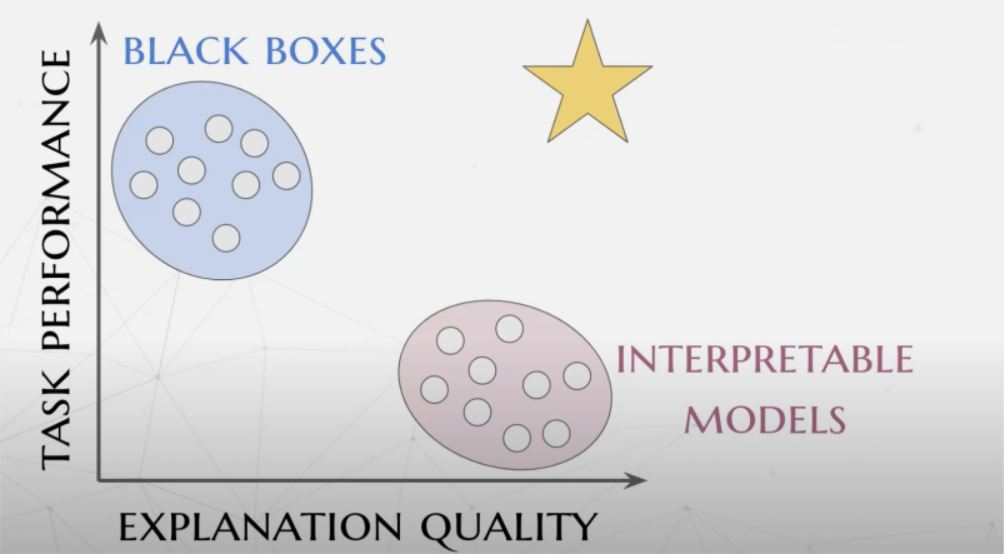
\includegraphics[width=0.5\linewidth]{Fig1.JPG}
     \caption{Can we build models that are both inherently interpretable and highly accurate?}
     \label{fig:f1}
 \end{figure}

\section{Concepts: The Building Blocks of Semantics}
A core idea in achieving interpretability is to decompose inputs into a set of concepts such as Figure \ref{fig:f2}. It means complex inputs can be understood through a set of human-understandable concepts that capture their semantic meaning.

\begin{itemize}
   \item Each input can be characterized by a collection of these concepts, which together represent its semantic meaning.
   \item For example, the concept slide provides a simple illustration: apple = red + round. This suggests that the semantic of an apple can be understood through the presence of the concepts ``red'' and ``round''.
   \item The paper \cite{dcr} formalizes this by suggesting that concept-based models learn a mapping from a concept space ($C$) to a task space ($Y$).
   \item When input features are not inherently meaningful (e.g., pixel intensities), a concept encoder ($g$) can map raw input features ($X$) to the concept space ($C$).
\end{itemize}

\section{Initial Idea: Logic Rules Based on Concepts}
A natural initial approach to building interpretable models is to describe each class using logical rules based on the presence or absence of these concepts e.g. logical AND of concepts.

\begin{itemize}
   \item One such idea is to represent each class as a logical AND of concepts. For instance: 
   \[ \text{Apple} = \text{Red} \land \text{Round} \]
   \item This representation is undoubtedly interpretable because the conditions for a class are explicitly stated in terms of human-understandable concepts.
   \item However, this crisp rule-based approach raises several important questions: 
   \begin{itemize}
       \item Where do these concepts come from?
       \item Where do the logical rules originate?
       \item Crisp, binary rules tend to be inaccurate in real-world scenarios due to the inherent complexity and variability of data.
   \end{itemize}
\end{itemize}

\begin{figure}
   \centering
   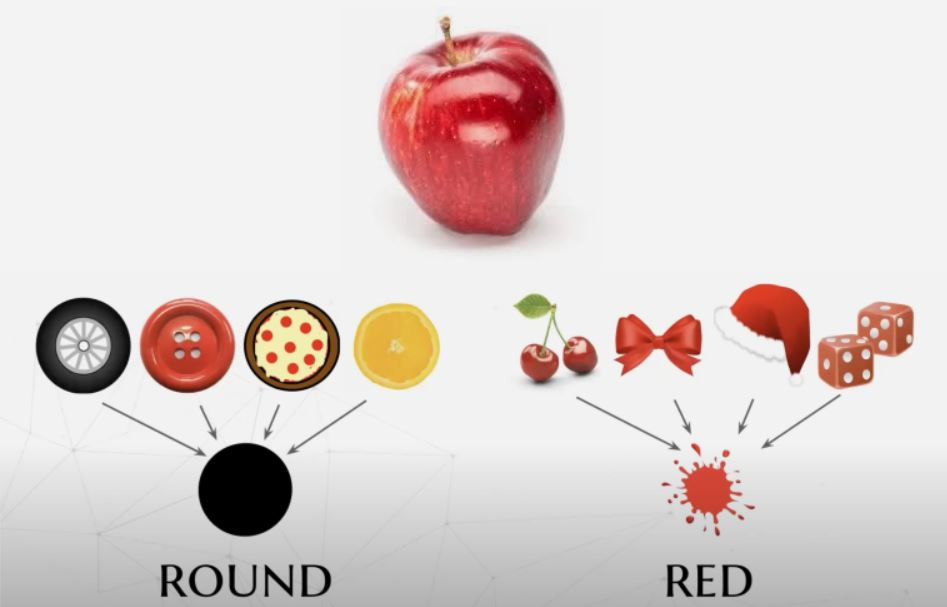
\includegraphics[width=0.5\linewidth]{Fig2.JPG}
   \caption{Decomposing inputs into a set of concepts.}
   \label{fig:f2}
\end{figure}

To address the first question, the idea of learning concepts from data arises. State-of-the-art concept-based models often rely on high-dimensional concept embedding representations to achieve high performance. However, these embeddings lack clear semantic meaning on individual dimensions, thus questioning the interpretability of the decision process. For example, a concept embedding for ``yellow'' as [2.3, 0.3, -3.5, ...] doesn't assign a specific meaning to each numerical value.

% \subsection{Concept Embeddings: Representing Concepts in a Vector Space}
\section{Concept Embeddings: Representing Concepts in a Vector Space}
Instead of treating concepts as binary (present or absent), we can represent them as embedding vectors in a high-dimensional space. (The paper \cite{dcr} notes that using only concept truth degrees can degrade task accuracy, which is why concept embeddings are often employed alongside them.)

\begin{itemize}
   \item For each concept $i$, we learn an embedding vector $c_i$. This vector can capture more nuanced aspects of the concept beyond a simple binary value.
\end{itemize}

The paper ``Concept Embedding Models: Beyond the Accuracy-Explainability Trade-Off'' by \citet{cem} proposes a novel family of concept bottleneck models (CEMs) that learn such interpretable high-dimensional concept representations. Figure \ref{fig:f2} in this paper (Figure 3 in here) illustrates the architecture of a Concept Embedding Model. For each concept $c_i$, CEM learns a mixture of two embeddings: $\hat{c}^+_i$ representing the active state of the concept and $\hat{c}^-_i$ representing the inactive state. A DNN $\psi(x)$ first learns a latent representation $h$ from the input $x$. This latent code is then fed into concept-specific fully connected layers $\phi^+_i(h)$ and $\phi^-_i(h)$ to generate $\hat{c}^+_i$ and $\hat{c}^-_i$ respectively:
% \begin{align*}
%    \hat{c}^+_i &= \phi^+_i(h) = a(W^+_i h + b^+_i) \\
%    \hat{c}^-_i &= \phi^-_i(h) = a(W^-_i h + b^-_i)
% \end{align*}
\begin{equation}
   \hat{c}^+_i = \phi^+_i(h) = a(W^+_i h + b^+_i)
\end{equation}
\begin{equation}
   \hat{c}^-_i = \phi^-_i(h) = a(W^-_i h + b^-_i)
\end{equation}
where $a(\cdot)$ is an activation function (e.g., leaky-ReLU). A scoring function $s([\hat{c}^+_i, \hat{c}^-_i]^T)$ then predicts the probability $\widehat{p_i}$ of concept $c_i$ being active:
% \[ \hat{p}_i = s([\hat{c}^+_i, \hat{c}^-_i]^T) = \sigma(W_s [\hat{c}^+_i, \hat{c}^-_i]^T + b_s) \]
\begin{equation}
   \hat{p}_i = s([\hat{c}^+_i, \hat{c}^-_i]^T) = \sigma(W_s [\hat{c}^+_i, \hat{c}^-_i]^T + b_s)
\end{equation}

The final concept embedding $\hat{c}_i$ is a weighted mixture of $\hat{c}^+_i$ and $\hat{c}^-_i$ based on $\widehat{p_i}$:
% \[ \widehat{c_i} = \hat{p}_i \hat{c}^+_i + (1 - \hat{p}_i) \hat{c}^-_i \]
\begin{equation}
   \widehat{c_i} = \hat{p}_i \hat{c}^+_i + (1 - \hat{p}_i) \hat{c}^-_i
\end{equation}

These concept embeddings are then concatenated to form a bottleneck $g(x) = \hat{c}$, which is passed to a label predictor $f$ for the downstream task.

\begin{figure}
   \centering
   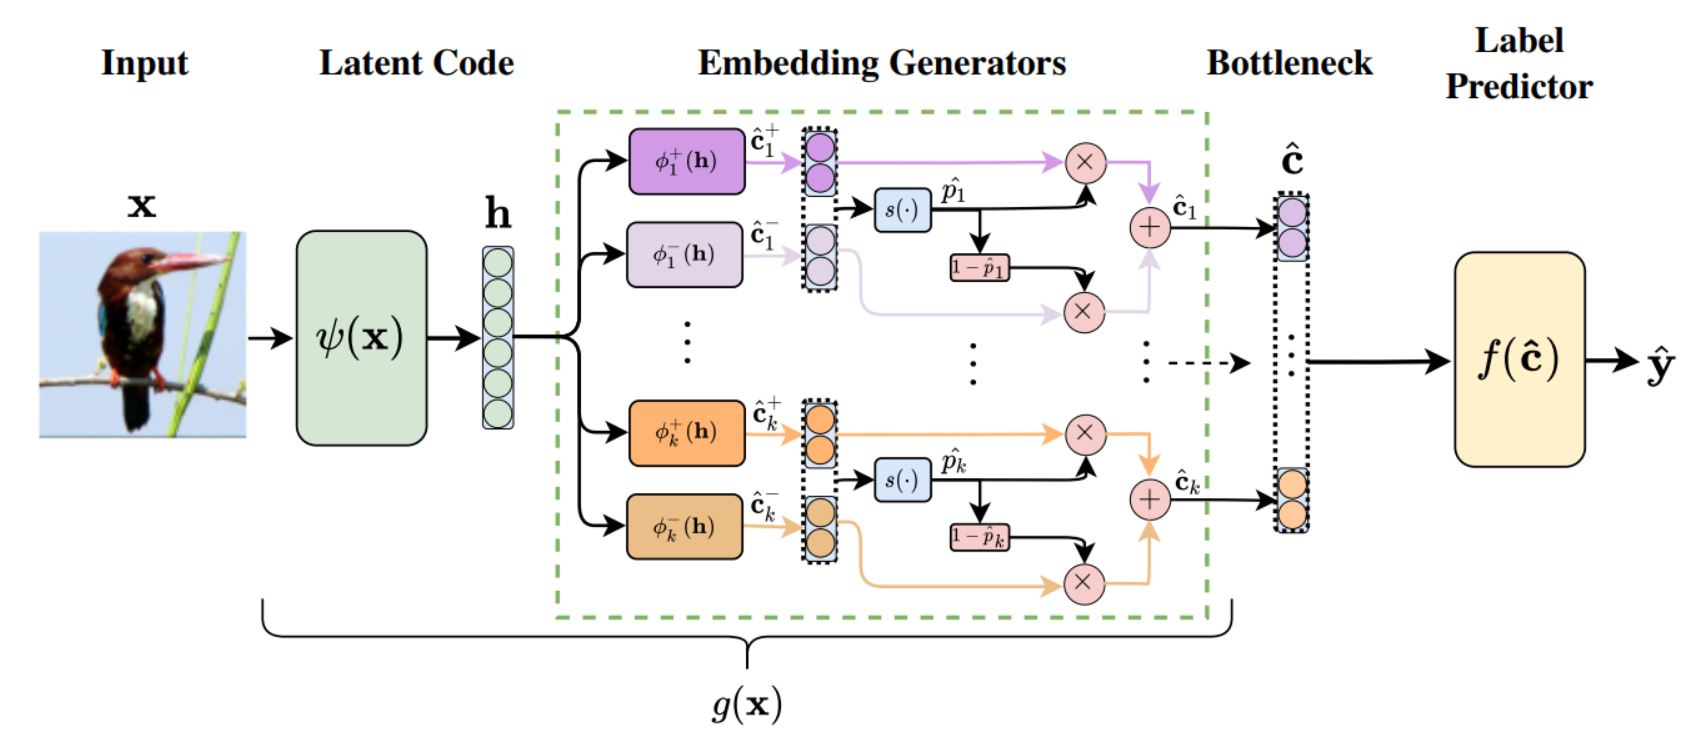
\includegraphics[width=0.8\linewidth]{Fig3.JPG}
   \caption{\textbf{Concept Embedding Model}: from an intermediate latent code $h$, we learn two embeddings per concept, one for when it is active (i.e., $\hat{c}^+_i$), and another when it is inactive (i.e., $\hat{c}^-_i$). Each concept embedding (shown in this example as a vector with $m = 2$ activations) is then aligned to its corresponding ground truth concept through the scoring function $s(\cdot)$, which learns to assign activation probabilities $\hat{p}_i$ for each concept. These probabilities are used to output an embedding for each concept via a weighted mixture of each concept's positive and negative embedding.}
   \label{fig:f3}
\end{figure}

\section{Learning Concept Existence: A Deep Model}
Building upon the idea of concept embeddings, we can train a deep model $g(x)$ that takes an input $x$ and outputs the existence (or, more accurately, the confidence of existence) of each concept $i$.

\begin{itemize}
   \item The output of $g(x)$ is in the form of a confidence score for each concept $i$. This confidence can be interpreted as a continuous truth value in the range, representing the degree to which the concept is present in the input.
\end{itemize}

\section{Rule Learning: Extracting Logical Relationships}
Now, how do we form rules based on these learned concept confidences? The ``Interpretable Neural-Symbolic Concept Reasoning'' paper \cite{dcr} proposes the Deep Concept Reasoner (DCR) to address this.

\begin{itemize}
   \item DCR uses neural networks to output the structure of a fuzzy logic rule.
   \item These rules are then executed on the truth degrees of the concepts to make a final prediction.
\end{itemize}

Specifically, for each predicted class $\widehat{y_j}$, DCR learns a rule with the syntax:
% \[ \hat{y}_j \Leftrightarrow \bigwedge_{i:r_{ji}=1} l_{ji} \quad \text{(Equation 1 in paper)} \]
\begin{equation}
   \hat{y}_j \Leftrightarrow \bigwedge_{i: r_{ji}=1} l_{ji} \quad \text{(Equation 1 in paper \cite{dcr})}
\end{equation}
This represents a logical equivalence where the prediction for class $j$ is true if and only if all relevant concept literals ($l_{ji}$) are true. 

where:
\begin{itemize}
   \item $l_{ji}$ is the literal of concept $c_i$ (either $c_i$ or $\lnot c_i$) representing its role for class $j$.
   \item $r_{ji} \in \{0,1\}$ indicates whether concept $c_i$ is relevant for predicting class $y_j$.
\end{itemize}

\begin{figure}
   \centering
   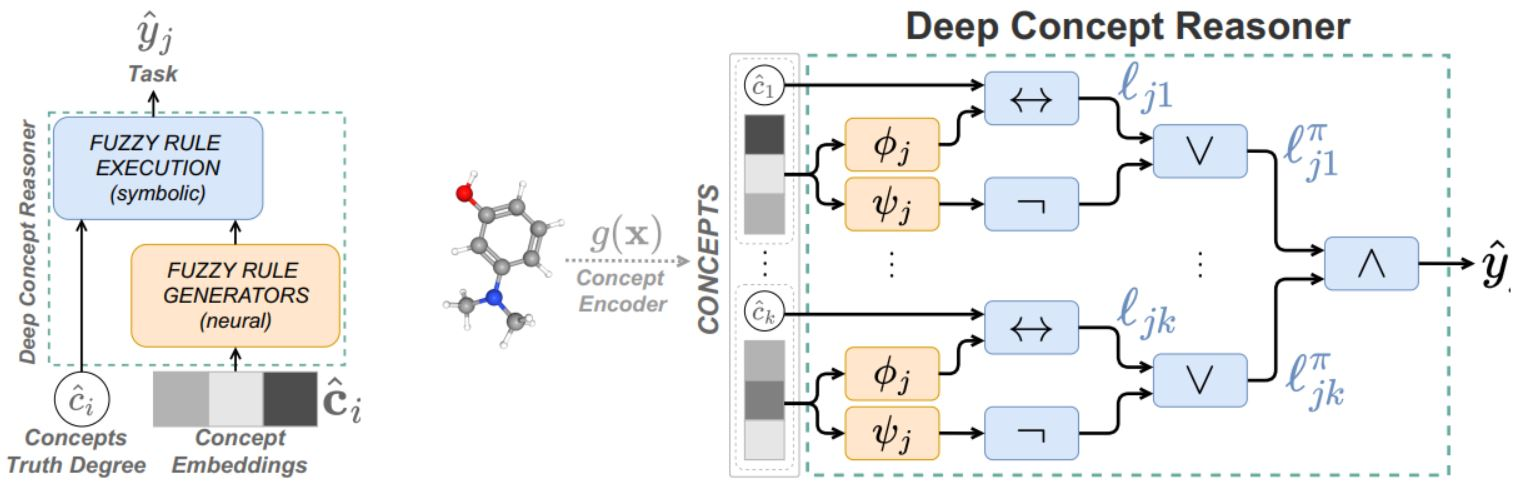
\includegraphics[width=0.8\linewidth]{Fig4.JPG}
   \caption{(left) Deep Concept Reasoner (DCR) generates fuzzy logic rules using neural models on concept embeddings. Then DCR executes the rule using the concept truth degrees to evaluate the rule symbolically. (right) Schema of DCR modules: first neural models $\phi$ and $\psi$ generate the rule, and then the rule is executed symbolically.}
   \label{fig:f4}
\end{figure}

DCR employs two neural modules for rule generation:
\begin{itemize}
   \item \textbf{Concept Role Generation}: A neural network $\phi_j: \R^m \rightarrow [0, 1]$ takes a concept embedding $c_i \in \R^m$ as input and determines its role (positive or negative) in the rule for class $j$. The truth degree of the literal $l_{ji}$ is then computed as: 
   % \[ l_{ji} = (\phi_j(\widehat{c_i}) \Leftrightarrow \widehat{c_i}) \quad \text{(Equation 2 in paper)} \]
   \begin{equation}
      l_{ji} = (\phi_j(\widehat{c_i}) \Leftrightarrow \widehat{c_i}) \quad \text{(Equation 2 in paper \cite{dcr})}
   \end{equation}
   Using the Gödel t-norm semantics, this becomes:
   % \[ l_{ji} = \min\{\max\{1-\phi_j(\widehat{c_i}), \widehat{c_i}\}, \max\{1-\widehat{c_i}, \phi_j(\widehat{c_i})\}\} \]
   \begin{equation}
      l_{ji} = \min\{\max\{1-\phi_j(\widehat{c_i}), \widehat{c_i}\}, \max\{1-\widehat{c_i}, \phi_j(\widehat{c_i})\}\}
   \end{equation}

   \item \textbf{Concept Relevance Generation}: Another neural network $\psi_j: \R^m \rightarrow [0, 1]$ takes a concept embedding $c_i$ and determines its relevance $r_{ji}$ for predicting class $j$. The truth degree of a relevant literal is: 
   % \[ l_{ji}^r = (\psi_j(\widehat{c_i}) \Rightarrow l_{ji}) = (\lnot \psi_j(\widehat{c_i}) \lor l_{ji}) \quad \text{(Equation 3 in paper )} \]
   \begin{equation}
      l_{ji}^r = (\psi_j(\widehat{c_i}) \Rightarrow l_{ji}) = (\lnot \psi_j(\widehat{c_i}) \lor l_{ji}) \quad \text{(Equation 3 in paper \cite{dcr})}
   \end{equation}
   Using the Gödel t-norm semantics, this becomes:
   % \[ l_{ji}^r = \max\{1-\psi_j(\widehat{c_i}), l_{ji}\} \]
   \begin{equation}
      l_{ji}^r = \max\{1-\psi_j(\widehat{c_i}), l_{ji}\}
   \end{equation}
   Note that Irrelevant concepts effectively have a truth degree of 1, making them neutral in the conjunction.
\end{itemize}

Finally, the task prediction $\widehat{y_j}$ is obtained by conjoining all the relevant literals using the Gödel t-norm (minimum):
% \[ \hat{y}_j = \bigwedge_{i=1}^k l^r_{ji} = \min_{i=1}^k \max\{1-\psi_j(\widehat{c_i}), l_{ji}\} \quad \text{(Equation 4 in paper adapted for Gödel t-norm)} \]
\begin{equation}
   \hat{y}_j = \bigwedge_{i=1}^k l^r_{ji} = \min_{i=1}^k \max\{1-\psi_j(\widehat{c_i}), l_{ji}\} \quad \text{(Equation 4 in paper \cite{dcr} adapted for Gödel t-norm)}
\end{equation}

You can see this process in Figure \ref{fig:f4} and an example in Figure \ref{fig:f5}.

\begin{figure}
   \centering
   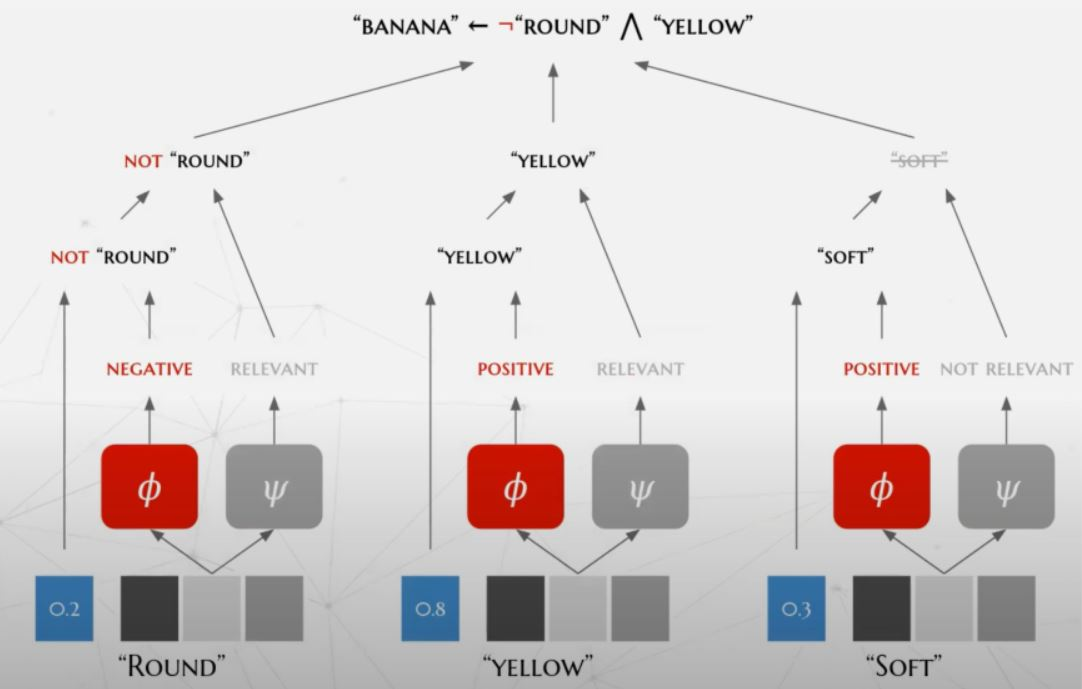
\includegraphics[width=0.5\linewidth]{Fig5.JPG}
   \caption{An example of rule learning.}
   \label{fig:f5}
\end{figure}

\section{Making it Differentiable: Continuous Logic}
To enable end-to-end training of such neuro-symbolic systems, it is crucial to make the discontinuous logical binary operators continuous.

\begin{itemize}
   \item Fuzzy logic provides a way to generalize Boolean logic by allowing truth values to range continuously between 0 and 1. For more details look at the Figure \ref{fig:f6}.
   \item T-norms (e.g., product, Gödel) generalize the logical AND operation ($\land$), and t-conorms generalize the OR operation ($\lor$). Negation ($\lnot$) is typically defined as $\lnot x = 1 - x$.
   \item By using differentiable t-norms and t-conorms, the entire rule execution process becomes differentiable, allowing the neural networks involved in rule generation to be trained using gradient descent. DCR, for instance, uses the Gödel t-norm in its implementation.
\end{itemize}

\begin{figure}
   \centering
   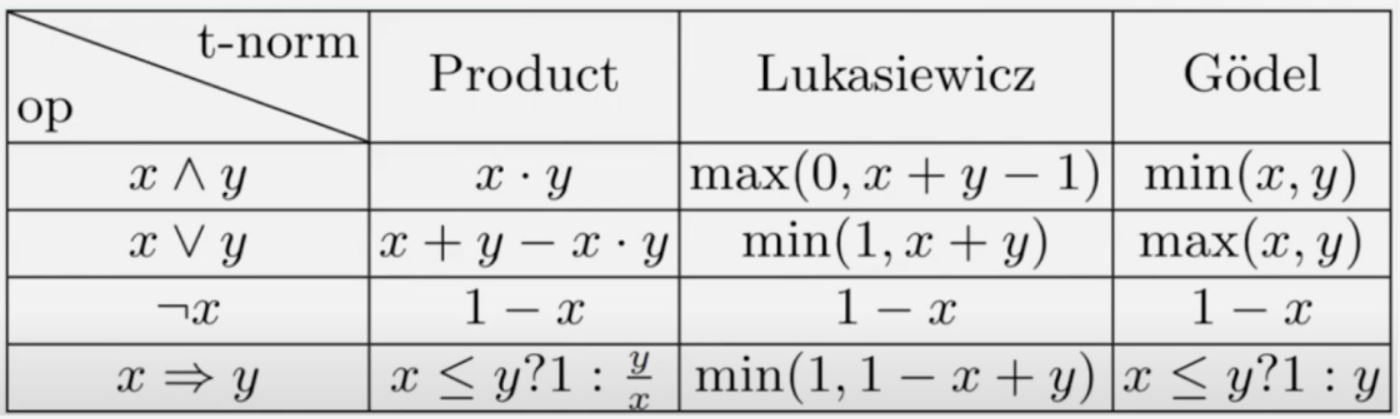
\includegraphics[width=0.5\linewidth]{Fig6.JPG}
   \caption{Some of the fuzzy logic operators.}
   \label{fig:f6}
\end{figure}

\section{Rule Parsimony and Fuzzy Semantics}
The paper \cite{dcr} discusses the importance of rule parsimony for human interpretability, aiming for simpler rules with only relevant concepts.

\begin{itemize}
   % \item DCR encourages parsimony by using a special activation function for the relevance network ($\psi_j$) based on a rescaled log-softmax. This introduces competition among concepts, favoring the selection of only the most relevant ones.
   \item DCR encourages parsimony by using a special activation function for the relevance network ($\psi_j$) based on a rescaled log-softmax. This introduces competition among concepts, favoring the selection of only the most relevant ones. The relevance score $r_{ji}$ for concept $i$ in class $j$ is computed as:
   
   % \begin{align*}
   %    \gamma_{ji} &= \log \left( \frac{\exp(\text{MLP}_j(\hat{c}_i))}{\sum_{i'=1}^k \exp(\text{MLP}_j(\hat{c}_{i'}))} \right) \\
   %    r_{ji} &= \psi_j(\hat{c}_i) = \sigma \left( \gamma_{ji} - \frac{1}{k} \sum_{i'=1}^k \gamma_{ji'} \right)
   % \end{align*}
   \begin{equation}
      \gamma_{ji} = \log \left( \frac{\exp(\text{MLP}_j(\hat{c}_i))}{\sum_{i'=1}^k \exp(\text{MLP}_j(\hat{c}_{i'}))} \right)
   \end{equation}
   \begin{equation}
      r_{ji} = \psi_j(\hat{c}_i) = \sigma \left( \gamma_{ji} - \frac{1}{k} \sum_{i'=1}^k \gamma_{ji'} \right)
   \end{equation}
   
   where $\text{MLP}_j$ is a multi-layer perceptron for class $j$, $\hat{c}_i$ is the concept embedding, and $\sigma$ is the sigmoid function. 
   This way, if the scores $\gamma_{ji}$ are uniformly distributed, then we expect the network $j$ to select half of the concepts. 

   % \item A temperature parameter ($\tau$) can be used to control the complexity of the rules, allowing users to bias towards simpler or more complex rules.
   \item A temperature parameter ($\tau \in [-\infty, \infty]$) can be used to control the complexity of the rules, allowing users to bias towards simpler or more complex rules. The parameter $\tau$ scales the mean term in the relevance computation:
   % \[ r_{ji} = \sigma\left(\gamma_{ji} - \frac{\tau}{k} \sum_{i'=1}^k \gamma_{ji'}\right) \]
   \begin{equation}
      r_{ji} = \sigma\left(\gamma_{ji} - \frac{\tau}{k} \sum_{i'=1}^k \gamma_{ji'}\right)
   \end{equation}
   Increasing $\tau$ produces more relevance scores closer to 1 (resulting in more complex rules), while decreasing $\tau$ produces more relevance scores closer to 0 (resulting in simpler rules).

   \item To maintain semantic validity and differentiability, DCR enforces the same semantic structure (Gödel t-norm) in both logic and neural operations.
\end{itemize}

\section{Experimental Evaluation and Key Findings}
The paper \cite{dcr} presents extensive experiments on various datasets to evaluate DCR's generalization, interpretability, and ability to generate counterfactual explanations. Key findings include:

\subsection{Generalization}
\begin{itemize}
   \item DCR outperforms state-of-the-art interpretable concept-based models in terms of task accuracy as depicted in Figure \ref{fig:f7}, especially when concept embeddings hold more information than just truth degrees.
   \item It can also generalize well even with concept shifts between training and testing.
   \item DCR also matches the accuracy of neural-symbolic systems trained with human rules on tasks like MNIST-Addition, even when learning rules from scratch.
\end{itemize}

\begin{figure}
   \centering
   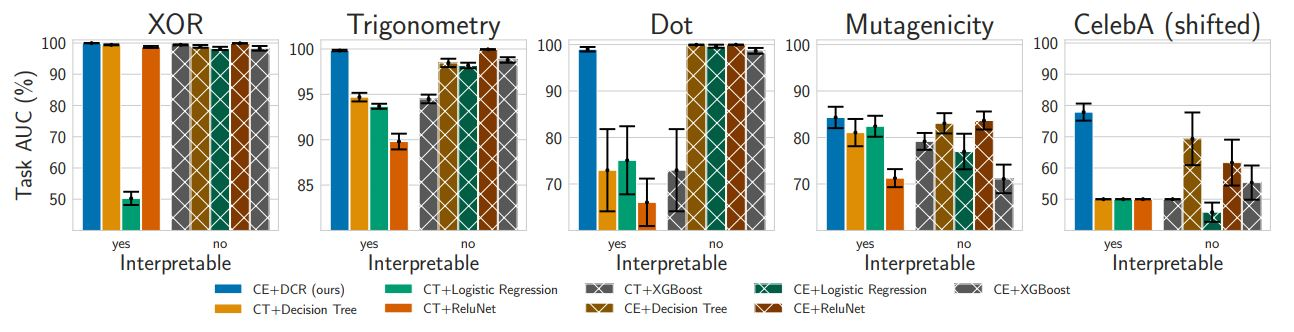
\includegraphics[width=1\linewidth]{Fig7.JPG}
   \caption{Mean ROC AUC for task predictions for all baselines across all tasks (the higher the better). DCR often outperforms interpretable
   concept-based models. CE stands for concept embeddings, while CT for concept truth degrees. Models trained on concept embeddings
   are not interpretable as concept embeddings lack a clear semantic for individual embedding dimensions.}
   \label{fig:f7}
\end{figure}

\subsection{Interpretability}
\begin{itemize}
   \item DCR discovers semantically meaningful logic rules that often match known ground truths in synthetic datasets. Some examples of dicovered logic rules versus ground-truth rules exist in the Table 1.
   \item Even in the absence of concept supervision (e.g., Mutagenicity), DCR rules can involve concepts related to domain knowledge (e.g., functional groups known for mutagenic effects).
   \item DCR rules are also stable under small perturbations of the input compared to local post-hoc explainers.
   \item Furthermore, DCR's transparent rules can explain prediction mistakes by identifying issues with concept predictions or rule relevance.
\end{itemize}

\begin{table}
   \centering
   \caption{Error rate of Booleanised DCR rules w.r.t. ground truth rules. Error rate represents how often the label predicted by a Booleanised rule differs from the fuzzy rule generated by our model. The error rate is reported with the mean and standard error of the mean. A full list of logic rules for MNIST is in Appendix H of the "Interpretable Neural-Symbolic Concept Reasoning" paper \cite{dcr}.}
   \begin{tabular}{lll}
   \toprule
   \textbf{GROUND-TRUTH RULE} & \textbf{PREDICTED RULE} & \textbf{ERROR (\%)} \\
   \midrule
   \multicolumn{3}{c}{\textbf{XOR}} \\
   \midrule
   $y_0 \leftarrow \neg c_0 \wedge \neg c_1$ & $y_0 \leftarrow \neg c_0 \wedge \neg c_1$ & \num{0.00} $\pm$ \num{0.00} \\
   $y_0 \leftarrow c_0 \wedge c_1$ & $y_0 \leftarrow c_0 \wedge c_1$ & \num{0.00} $\pm$ \num{0.00} \\
   $y_1 \leftarrow \neg c_0 \wedge c_1$ & $y_1 \leftarrow \neg c_0 \wedge c_1$ & \num{0.02} $\pm$ \num{0.02} \\
   $y_1 \leftarrow c_0 \wedge \neg c_1$ & $y_1 \leftarrow c_0 \wedge \neg c_1$ & \num{0.01} $\pm$ \num{0.01} \\
   \midrule
   \multicolumn{3}{c}{\textbf{Trigonometry}} \\
   \midrule
   $y_0 \leftarrow \neg c_0 \wedge \neg c_1 \wedge \neg c_2$ & $y_0 \leftarrow \neg c_0 \wedge \neg c_1 \wedge \neg c_2$ & \num{0.00} $\pm$ \num{0.00} \\
   $y_1 \leftarrow c_0 \wedge c_1 \wedge c_2$ & $y_1 \leftarrow c_0 \wedge c_1 \wedge c_2$ & \num{0.00} $\pm$ \num{0.00} \\
   \midrule
   \multicolumn{3}{c}{\textbf{MNIST-Addition}} \\
   \midrule
   $y_{18} \leftarrow c_9' \wedge c_9''$ & $y_{18} \leftarrow c_9' \wedge c_9''$ & \num{0.00} $\pm$ \num{0.00} \\
   $y_{17} \leftarrow c_9' \wedge c_8''$ & $y_{17} \leftarrow c_9' \wedge c_8''$ & \num{0.00} $\pm$ \num{0.00} \\
   $y_{17} \leftarrow c_8' \wedge c_9''$ & $y_{17} \leftarrow c_8' \wedge c_9''$ & \num{0.00} $\pm$ \num{0.00} \\
   \bottomrule
   \end{tabular}
\end{table}

\subsection{Counterfactual Explanations}
\begin{itemize}
   \item DCR enables the discovery of simple counterfactual examples by leveraging the learned logic rules to identify the most relevant concepts to perturb.
   \item Its confidence in predictions drops quickly when relevant concepts are perturbed.
\end{itemize}

\pagebreak

\section{Global and Counterfactual Explanations}
DCR provides mechanisms for both global and local (counterfactual) explanations.

\begin{itemize}
   \item \textbf{Interpreting Global Behaviour}: By collecting and Booleanizing the fuzzy rules generated by DCR on the training data and aggregating them with a global disjunction ($\lor$), a single logic formula ($\hat{y}^C_j$) can be obtained to represent the global decision process for each class $j$.
   \item \textbf{Counterfactual Explanations}: The learned logic rules directly reveal the key concepts for a prediction, facilitating the extraction of simple counterfactual explanations. 
   \begin{itemize}
       \item Counter-examples ($x^\star$) are generated to be as close as possible to the original sample ($|x - x^\star| < \epsilon$).
       \item Concepts in the rule are ranked according to their relevance scores.
       \item Starting with the most relevant concept, their truth values are inverted until the model's prediction changes, providing a counterfactual explanation.
   \end{itemize}
\end{itemize}

\section{DCR and Neuro-Symbolic Architecture}
The concept of using neural networks to generate and execute symbolic rules falls under the umbrella of Neuro-Symbolic AI.

\begin{itemize}
   \item The slide mentions that DCR (Deep Concept Reasoner) is a method based on Neural-Symbolic approaches.
   \item It provides examples of other Neuro-Symbolic architectures: 
   \begin{itemize}
       \item \textbf{Neural Theorem Prover}: Constructs a neural network from an AND-OR proof tree generated from knowledge base rules and terms.
       \item \textbf{Logic Tensor Networks (LTNs)}: Another category that falls under Neural-Symbolic architectures. LTNs use tensor representations for logical terms and fuzzy predicates, allowing logical reasoning within a neural network framework.
   \end{itemize}
\end{itemize}

\section{Limitations and Future Directions}
The final slide prompts a brainstorming session to discuss the limitations of this work and how to improve it. Some potential limitations and areas for improvement based on papers could include:

\begin{itemize}
   \item \textbf{Complexity of Learned Rules}: The complexity of DCR rules might increase in certain scenarios. Exploring methods to encourage simpler and more generalizable rules could be beneficial.
   \item \textbf{Requirement for Concept Embeddings}: DCR relies on the existence of concept embeddings, which might require concept-annotated datasets or effective concept discovery methods. Investigating how to learn meaningful concepts and their embeddings more efficiently, potentially in an unsupervised or weakly supervised manner (as explored in the MNIST addition experiment in "Interpretable Neural-Symbolic Concept Reasoning" paper \cite{dcr}), is important.
   \item \textbf{Global Interpretability}: While DCR provides interpretable rules for individual predictions, its global behavior, represented by the disjunction of all learned rules, might still be complex to fully grasp. Developing techniques for more concise and understandable global explanations could be valuable.
   \item \textbf{Scalability to a Large Number of Concepts}: The number of concepts can impact the complexity of the rule learning process. Exploring methods to handle a large vocabulary of concepts efficiently would be relevant.
   \item \textbf{Robustness to Noisy or Incomplete Concept Information}: Investigating how these neuro-symbolic models perform when the concept information is noisy or incomplete, and developing mechanisms to handle such uncertainty, is crucial for real-world applications. The ``Concept Embedding Models'' paper \cite{cem} shows that CEMs can handle scarce concept supervision.
   \item \textbf{Ethical Considerations}: Interpretability is linked to ethical AI. Further research should consider the societal implications of these interpretable models and how they can contribute to more trustworthy and responsible AI systems.
\end{itemize}

\section{Conclusion}
The Deep Concept Reasoner (DCR) represents a significant advancement in interpretable concept-based models. By learning weighted logic rules from concept embeddings and executing them on concept truth degrees in a differentiable manner, DCR achieves a compelling balance between accuracy and interpretability. The experimental results demonstrate its superior performance compared to other interpretable models, its ability to discover meaningful rules, and its utility in generating counterfactual explanations. While some limitations exist regarding global interpretability and the need for concept embeddings, DCR marks a substantial step forward in the field of explainable AI.

% \section*{References}
% \begin{thebibliography}{9}

% \bibitem{cem}
% Espinosa Zarlenga, M., Barbiero, P., Ciravegna, G., Marra, G., Giannini, F., Diligenti, M., ... \& Weller, A. (2022). 
% \textbf{Concept Embedding Models: Beyond the Accuracy-Explainability Trade-Off}. 
% Advances in Neural Information Processing Systems, 35, 21400-21413. \\
% \url{https://arxiv.org/abs/2209.09056} 

% \bibitem{dcr}
% Barbiero, P., Ciravegna, G., Giannini, F., Zarlenga, M. E., Magister, L. C., Tonda, A., ... \& Jamnik, M. (2023). 
% \textbf{Interpretable Neural-Symbolic Concept Reasoning}. 
% arXiv preprint arXiv:2304.14068. \\
% \url{https://arxiv.org/abs/2304.14068}

% \end{thebibliography}

\bibliographystyle{plainnat}
\bibliography{references} % references.bib file

\end{document}